\section{QGIS Plugins}\index{plugins}

% when the revision of a section has been finalized, 
% comment out the following line:
\updatedisclaimer

QGIS has been designed with a plugin architecture. This allows new 
features/functions to be added to the application. Many of the features in 
QGIS are actually implemented as core or external plugins.\index{plugins!types} 

A QGIS core plugin is maintained by the QGIS Development Team 
and is part of every QGIS distribution (see Section \ref{sec:core_plugins}).

An external plugin is stored in an external svn repository and maintained 
by the individual author. It can be added to QGIS with the Plugin installer. 
You find more information about external plugins in Section 
\ref{sec:external_plugins}.

\subsection{Finding and Installing a Plugin}
When you install QGIS, all of the core plugins are included (see chapter \ref{sec:core_plugins}). \index{plugins!installing}

Typically user-contributed plugins are distributed in source form and require compiling.
For instructions on building and installing a user-contributed plugin, see the documentation included with the plugin.

\subsection{Managing Plugins}\label{sec:managing_plugins}
\index{plugins!managing} Managing plugins consists of loading or unloading them from QGIS.
Loaded plugins are "remembered" when you exit the application and restored the next time you run QGIS.

To manage plugins, open \mainmenuopt{Plugins} > \dropmenuopttwo{mActionShowPluginManager}{Plugin Manager...}
\index{plugins!manager}The Plugin Manager displays all the available plugins and their status (loaded or unloaded).
Figure \ref{fig:pluginmanager} shows the Plugin Manager dialog.

%\begin{figure}[ht]
%   \begin{center}
%   \caption{Plugin Manager}\label{fig:pluginmanager}\smallskip
%   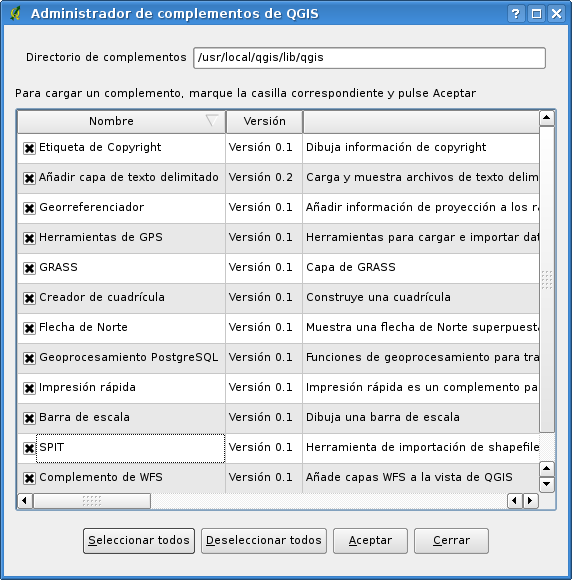
\includegraphics[clip=true, width=14cm]{pluginmanager2}
%\end{center}  
%\end{figure}

Typically all QGIS plugins are installed in the same location.
This location is shown in the Plugin Directory text field.
You can tell QGIS to load plugins from another location by specifying a different directory.

\begin{Tip}\caption{\textsc{Crashing Plugins}}\index{crashes}
\qgistip{If you find that QGIS crashes on startup, a plugin may be at fault.
You can stop all plugins from loading by editing your stored settings file (see \ref{subsec:gui_options} for location).
Locate the plugins settings and change all the plugin values to false to prevent them from loading.
\nix {For example, to prevent the Delimited text plugin from loading, the entry in \$HOME/.config/QuantumGIS/qgis.conf on Linux 
should look like this:\usertext{Add Delimited Text Layer=false}.}
\normalfont 
Do this for each plugin in the [Plugins] section.
You can then start QGIS and add the plugins one at a time from the Plugin Manger to determine which is causing the problem.
}
\end{Tip} 

\subsection{Data Providers}\index{data providers}

Data Providers are "special" plugins that provides access to a data store.
By default, QGIS supports PostGIS layers and disk-based data stores supported by the GDAL/OGR library (Appendix \ref{appdx_ogr}).
A Data Provider plugin extends the ability of QGIS to use other data sources.

Data Provider plugins are registered automatically by QGIS at startup.
They are not managed by the Plugin Manager but are used behind the scenes when a corresponding data type is added as a layer in QGIS.

